\begin{frame}{Problem description}%
    \begin{columns}[T,onlytextwidth]%
        \begin{column}[T]{0.48\textwidth}%
            Balancing the trunk on long legs is a major challenge in bipedal walking.\\
            Task Description:
            \begin{enumerate}
                \item Quantify and analyze different trunk pitch control strategies.
                \item Implement relevant controllers in JenaFox simulation.
                \item Evaluate selected approaches on robotic test environment.
            \end{enumerate}%
        \end{column}%
        \begin{column}[T]{0.48\textwidth}%
            \begin{figure}[htb]%
                \centering%
                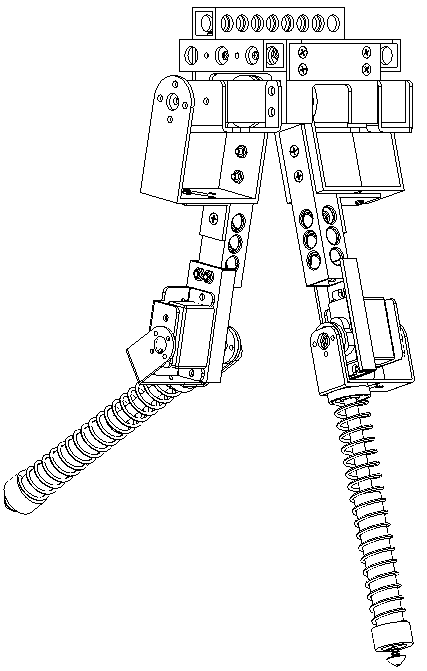
\includegraphics[width=0.5\textwidth]{figures/jena-fox-wireframe-transparent-black.png}%
                \caption{JenaFox Bipedal Walking Robot.}%
                \label{fig:jenafox}%
            \end{figure}%
        \end{column}%
    \end{columns}%
\end{frame}%
%
\note[itemize]{%
    \item Bipedal walking: Complex task, highly dynamical gait that involves flight phase, during which no force can be applied to environment
    \item Among others, one of the biggest challenges: balance torso on long legs
    \item Analyze, implement, evaluate (JenaFox on left)
}%
%